\chapter{Existing Discussion on Research Automation}
\label{chapter-literature-review}

This chapter will focus specifically on the automation of science. Attempts to automate science began soon after the advent of computers. Until then, humans had developed science by describing experiences (primary science) and by making predictions through the construction of theories (secondary science). With the advent of computers came simulation science (third science), which uses computers to automate complex scientific computations, and data-driven science (fourth science), which automates the discovery of laws from large-scale data \cite{hey2009fourth}. Within the individual academic discipline ``X,'' the third science gave rise to the field of \textit{Computational-X} and the fourth science gave rise to the field of \textit{X-infomatics}, leading to the automation of entire academic disciplines.

In particular, the field of \textit{AI for Science}, which automates scientific research with AI, has expanded rapidly and achieved significant results due to the remarkable development of machine learning technology since the 2010s. Automation of scientific research with AI, including logical AI, has been an area of interest since the advent of AI \cite{langley1987scientific}, and the remarkable performance of deep neural networks has now made almost all scientific fields more or less influenced by AI. In particular, recent developments in large-scale language modeling have significantly solved one of the biggest barriers to AI in the past, namely, language processing, and are creating a major trend toward automation in all fields of science.

While there have been some excellent review articles and perspective papers on previous efforts to automate research, there have not yet been many reviews that deal with these research automation efforts in a shallow or even conservative manner. Therefore, this chapter provides the most comprehensive review possible of research on research automation to date.

The field related to research automation is vast. While it is not possible to cover all of them, we aim to present as comprehensive an introduction as possible. For this reason, the review of each individual field will be limited to a brief overview. We will introduce survey papers and other literature in those fields, and those who wish to understand more advanced discussions should refer to those references.

In the following, we will present the past efforts of mankind related to research automation, paying attention to what level of general ``task'' each research automation is oriented toward. This is because efforts to automate research can be interpreted as automating a set of tasks in the research process, or acquiring the ability to do so. Note that the level of generality treated here is naturally not absolute, but is set for convenience. Also, please keep in mind that this classification is for classifying human research activities, so humans are only assumed as the subject of the research. After introducing each effort, we will position these efforts in light of the formulation of the knowledge production process that this paper has dealt with.

\textcolor{red}{CAUTION: We have not read all of the literature in detail and it may contain errors. We will continue to update this paper, but if you find errors, please contact us or throw us a pull request.}

\section{Level of Generality of Task/Skill}
The first and most versatile ability is the ability to perform any task a human being can perform. This includes, for example, the ability to think, to manipulate language, and to act. Second, there are abilities that are required for any research. These include the ability to ask questions, generate hypotheses, and test hypotheses, as explained in Chapter 2. The ability to manipulate the scholarly literature and to search for information are also included in these abilities. This is because research is the activity of producing knowledge from arbitrary inputs, and information retrieval is essential for obtaining inputs, and manipulation of the academic literature is essential for processing and outputting these inputs. So far, this is the capability required for all research.

Next, there are fields of study that involve some form of quantity in order to do the research. If there are basic quantities involved, whether in the natural or social sciences, then this is the field. These research fields require the ability to manipulate mathematics in some form. In those fields that require the use of empirical methods, which are research methods for generating and analyzing data, you need to be able to use statistics and data analysis.

And there are abilities that are universally needed within each discipline, such as natural sciences, social sciences, and humanities. For example, in the natural sciences, the ability to perform experiments that interact with the physical world is an essential skill in a very broad range of natural sciences.

Below that, the generality of tasks and the ability to acquire them gradually narrows down to abilities that are widely needed within each discipline as a whole, such as physics, chemistry, biology, and medicine, and then to abilities needed in even smaller disciplines, such as condensed matter physics, organic chemistry, and molecular biology, and so on.

Fig. \ref{fig:generality_level} represents the hierarchical structure of generality of tasks we have discussed above. Of course, in actual research, the disciplines are closely related to each other, and such a hierarchical structure is not perfect. What we want to emphasize here is that there are differences in the degree of generality of the technologies to be automated and the capabilities to acquire them, and that each automation effort can be considered distinct in terms of its degree of generality. In the following, we will review the automation efforts of previous studies, focusing on these differences. To emphasize again, this chapter will focus on automation efforts in research related to science in the narrow sense, i.e., the natural sciences.


\begin{figure}[htb]
    \centering
    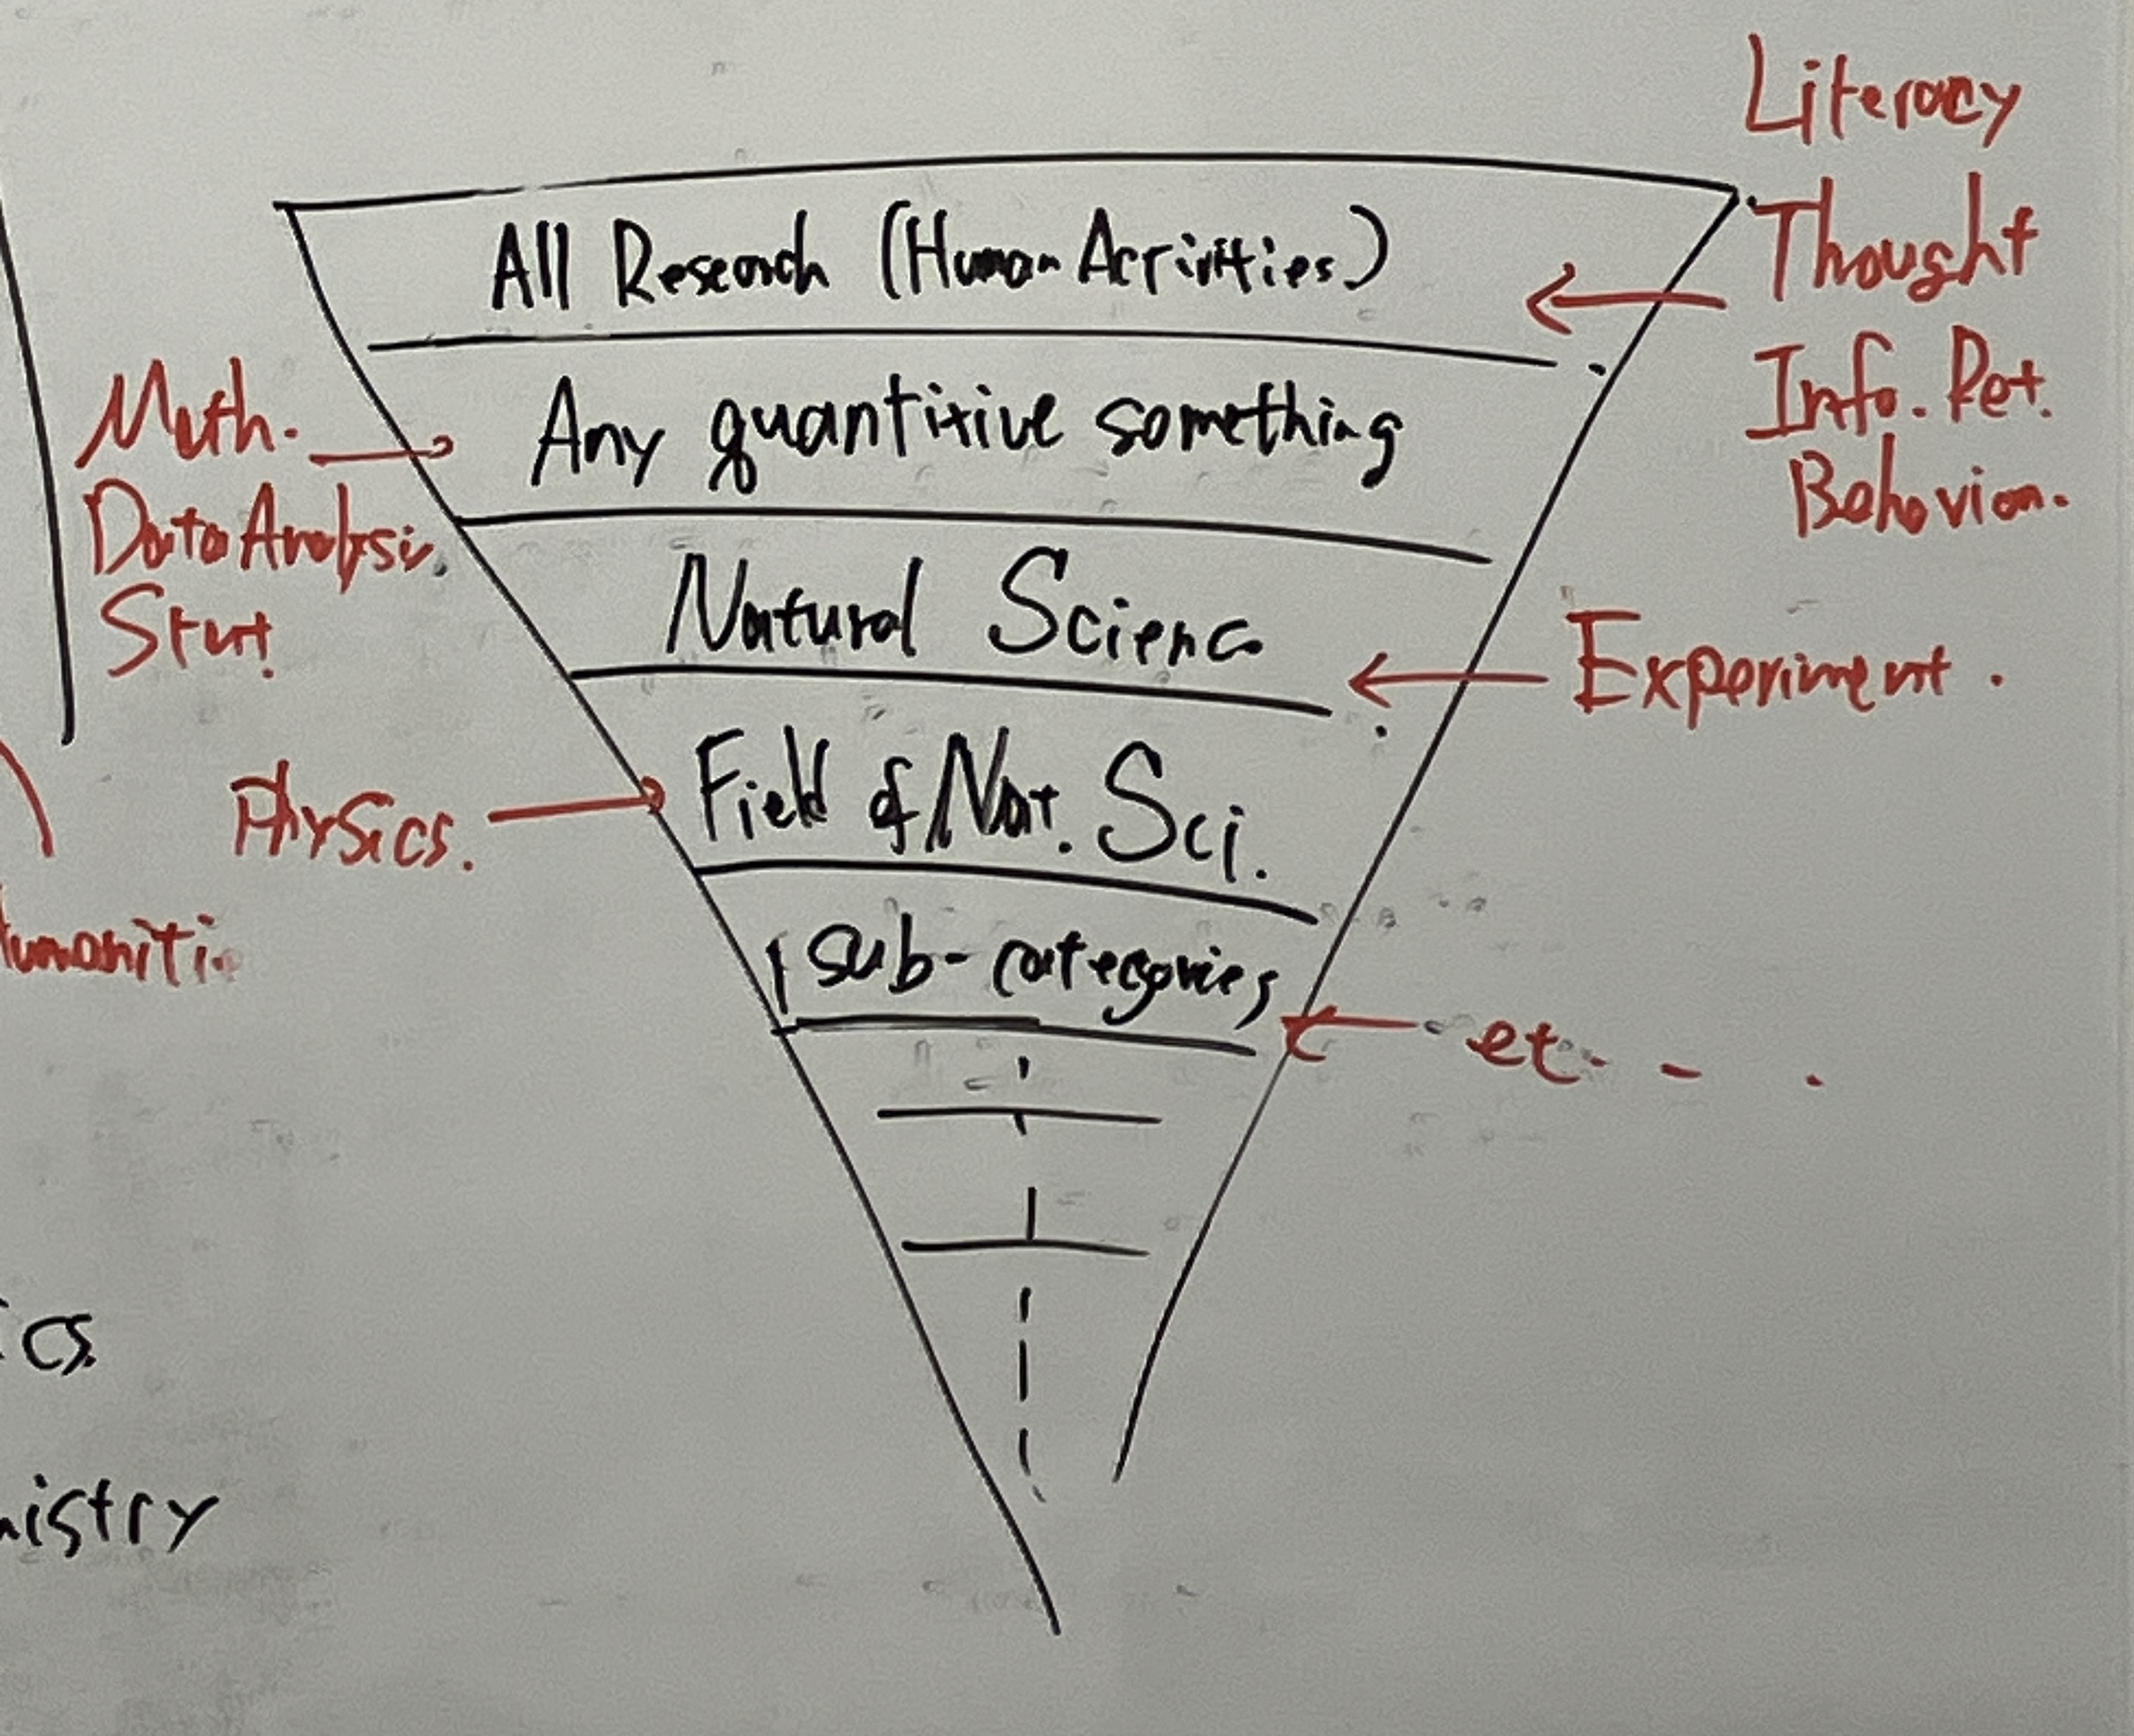
\includegraphics[width=\linewidth]{figs/generality_level.jpg}
    \caption{Caption}
    \label{fig:generality_level}
\end{figure}

\section{Automation of Tasks for Diverse Field of Research}

\subsection{Scholarly Document Processing}
\textit{Scholarly document processing} is a general term for research on automated processing related to scholarly articles and has been studied as part of natural language processing, text mining, and information retrieval.

\textcolor{red}{TODO: Skip for now. Need reconstruction because many of the issue discussed below are no more issue for research automation. Most of these will moved to Appendix}

\subsubsection{Searching}

Firstly, let us mention academic search engines that provide features to help researchers find relevant papers from a vast amount of literature \cite{googlescholar,semanticscholar,dblp,pubmed,citeseerx}. 

Specialized search systems have also been proposed for specific purposes. For example, some studies have been proposed systems to discover studis in other domeins \cite{kang2022augmenting}, difficulties, limitations and emerging hypotheses \cite{lahav2022search}, and author homepages \cite{patel2021author}. Also, in response to the COVID pandemic, several systems have emerged in recent times to search for COVID-19 related papers \cite{hope2020scisight}.

Instead of searching for papers manually, there are approaches that directly recommend papers to researchers. In practice, it is common for the specific aspects of academic papers that researchers want to compare to vary depending on the situation and research field. Therefore, researchers have invented the method allowing comparison in certain aspect of papers \cite{ostendorff2020aspect} and tailored to some particular research area \cite{breitinger2022recommending}. Also, some researchers study recommendation of authors instead of papers \cite{portenoy2022bursting}. A comprehensive summary of classical research on paper recommendation can be found in \cite{bai2019scientific}.

\subsubsection{Reading}
The majority of research on automation in research pertains to automating operations related to papers. Specifically, research on information extraction from papers constitutes the majority. Here, \textit{reading} refers to extracting information from a paper.

Several methods specialized in extracting specific information have been proposed. For instance, there are studies for extracting mathematical expressions \cite{greiner2020math,madisetty2021neural}, measure \cite{harper2021semeval,kohler2021s}, tabale and figure \cite{shen2022vila,hashmi2021current,zhuang2022resel,yamamoto2021visual}, dataset \cite{hou2019identification,kumar2021dataquest,prasad2019dataset}, and results \cite{kardas2020axcell}.

There are also studies that focus not on information extraction, but on determining the meaning of sentences written in papers. One representative example is research on citation classification, which involves understanding the intent behind the cited text \cite{pride2019act,kunnath2021meta,kunnath2022dynamic,kunnath2022act2,lauscher2021multicite}. Another example is topic/theme classification, which detect the main topic of the paper \cite{sadat2022hierarchical,mendoza2022benchmark,salatino2022cso}.

One of the most heavily researched areas of information extraction from scientific papers is summarization. Some studies propose methods to generate the contribution of a paper \cite{hayashi2020s}, scientific claims \cite{wright2022generating}, and lay summarization \cite{goldsack2022making}. Other studies have attempted to create better paper summaries using citation graph \cite{chen2022scientific,an2021enhancing}, or propose the summarization system \cite{erera2019summarization}.

Many of the earlier summarization studies only used limited information such as abstracts. In recent years, there have been proposed studies that generate summaries by reading the entire paper \cite{subramanian2019extractive,qi2022sapgraph,dong2020discourse,tretyak2020combination}.

Also, the number of papers has increased dramatically, and the time available for obtaining information from a single paper has become increasingly limited. Thus, some studies propose the methods to generate extremely short summaries, such as TLDR \cite{cachola2020tldr} and key phrases \cite{boudin2021keyphrase,garg2021keyphrase}.

To advance these summarization studies, some studies propose datasets \cite{yasunaga2019scisummnet,bastan2022sume} and annotation platforms \cite{el2022platform} for paper summarization. 

The early research on paper summarization, which was conducted relatively early, is well summarized in \cite{altmami2022automatic}. If you are interested, please also refer to this paper.

Up to this point, we have described methods that assume extracting specific information or summarizing papers. In contrast, there are studies that issue queries in natural language to retrieve desired information from papers. This has been formalized as a question-answering task, a more general problem setting \cite{lu2022learn,ruggeri2022argscichat,saikh2022scienceqa}. 

In the field of question-answering for academic papers, some web services have gained attention for its high performance \cite{elicit,scispace}. Elicit use large language models and compose them to write \textit{compositional language model programs}. Ought \cite{ought}, the provider of Elicit, publish the instructions of how to write compositional language model programs \cite{primer2022}. Also, they disclose how to update their system with their idea of \textit{process supervision} \cite{reppert2023iterated}. Therefore, for those who are interested in question-answering systems for scientific papers, we strongly recommend reading these papers and documents.

Lastly, many tools have been proposed to assist researchers in reading papers. These studies highlight rhetorical roles \cite{fok2023scim,lauscher2018arguminsci}, generate description to terminologies \cite{august2022generating,head2021augmenting,murthy2022accord}, simplify texts for non-experts \cite{august2022paper,jeblick2022chatgpt}, and allow interaction \cite{kang2022threddy,elicit,scispace}.

\subsubsection{Writing}
Research is the act of producing a novel knowledge on top of prior studies. The apt incorporation of previous literature and elucidation of the distinctions between the proposition and previous studies are essential. Consequently, some researchers have investigated to generate comparative arguments \cite{yu2022scientific} and others have studied to generate citation texts \cite{arita2022citation,gu2022controllable,wang2021autocite,xing2020automatic,funkquist2022citebench}. Additionally, several studies exist that, instead of directly producing text, aspire to assist in the writing process by recommending relevant literature for inclusion as citations \cite{farber2020citation,zhang2020dual,duma2019contextual,farber2018cite,gosangi2021use}. Furthermore, there exist investigations aimed at automating systematic reviews writing \cite{dones2022systematic}.

Scholarly articles are structured documents. This structural property enables researchers to generate texts per sections. Thereafter, 
researchers have endeavored to generate, for example, abstract \cite{kumarasinghe2022automatic,gao2022comparing,wang2019paperrobot}, related works \cite{li2022automatic,shah2021generating}, table description in result section \cite{moosavi2021scigen,moosavi2021learning}, conclusion, and future work \cite{wang2019paperrobot}. Wang et al. propose to generate even next research's probable title \cite{wang2019paperrobot}.

Similar to the situation with reading, proposals have emerged for systems to support writing \cite{narimatsu2021task}, as well as for datasets to train text generation \cite{chen2021scixgen}. In recent times, some researchers try to have GPT series to write academic papers \cite{transformer2022can}. 

\subsection{Peer Review}
Many studies have tried to automate peer review generation \cite{thelwall2019artificial,li2019generating,schulz2022future,yuan2022can,yuan2022kid,lin2021automated1,lin2021automated2,kumar2022investigations,bharti2022can,uban2021generating,wang2020reviewrobot}. While not generating peer reviews directly, studies focused on automating research paper assessment  can be said to be related to the peer review automation. \cite{kousha2022artificial,li2020multi,huang2018deep}. These studies have proposed the method to assess the quality \cite{thelwall2022predicting,thelwall2022can}, novelty \cite{pelletier2022novelpy,amplayo2019evaluating,shibayama2020measuring}, soundness \cite{cabanac2022decontamination}, and significance \cite{zong2022citation,xia2023review,soni2022predicting,manghi2021new,soni2021follow,van2020schubert,mckeown2016predicting}.

These investigations concern the automation of processes occurring subsequent to a manuscript's arrival at the hands of reviewers. Conversely, researchers also have investigated the automation before that process, such as determining the appropriate journal for submission \cite{michail2023journal} and assigning the reviewers \cite{zhao2022reviewer}.

While not centered on automation, certain studies engage in the scientific analysis of the review process \cite{shah2022challenges,verma2021attend,bharti2022confident,bharti2022betterpr,verma2022lack,kennard2022disapere}. These investigations serve to enhance our understanding of the nature of peer review and, in turn, provide valuable insights for the design of more effective automated review methodologies. 

\subsection{Cognitive }

\section{Automation of Tasks for Diverse Fields of Science}
% There are prerequisite competencies and knowledge required to conduct scientific research. And the question of how to acquire such abilities has been one of the major concerns of AI research for science. Therefore, we will first introduce these research areas. In particular, we will present research on processing scientific literature and understanding scientific knowledge.

\subsection{Automated Theorem Proving}

The automation of mathematical proof, \textit{automated theorem proving} (ATP) , has been studied for a long tius. Recently several effort has come up to improve ATP by using machine learning, and especially deep learning. The 
 early seminal work is led by Schulz \cite{schulz2001learning} and Urban \cite{urban2004mptp,urban2008malarea}. The first work applying deep learning to ATP is \cite{irving2016deepmath}. Subsequently, numerous studies have emerged on Automated Theorem Proving (ATP) using deep learning \cite{bansal2019holist}. Recent studies on this topic are well organized in the following paper, so we recommend reading it if interested \cite{rabe2021towards}.
 % TODO: more organized literature review

 While research has been accumulated on ATP, there is still not much research done on the automated theorem discovery with a few exceptions \cite{gao2014systematic}. In recent years, attempts have been made to help humans to find mathematical conjectures \cite{davies2021advancing} and
 automatically generate mathematical conjectures \cite{raayoni2021generating}  using machine learning.

% \subsection{Understanding Scientific Knowledge}

% \subsection{AI for Science}

TODO

\subsection{Scientific Language Models/Foundation Models}
In order for us to do scientific research, we must have learned prior knowledge about science. Therefore, research has been done to teach or incorporate such scientific knowledge and assumptions into machine learning models.

One of the most popular approaches today is to create foundational models in science. A foundational model is a pre-trained model that can be adapted to extremely generic downstream tasks. In particular, because language is an extremely general-purpose interface and because language models have developed by leaps and bounds, large-scale language models are now predominantly trained on vast amounts of textual data.

In science, scientific large-scale language models have also been developed by training huge amounts of scientific texts, including textbooks and papers \cite{taylor2022galactica}.
% \cite{beltagy2019scibert,singh2022scirepeval,nadkarni2021scientific,cohan2020specter,gupta2022matscibert,taylor2022galactica}.

% \subsubsection{Scientific Language Models}

Whether engaging in reading or writing, the presence of a system that comprehends natural language is indispensable. In recent years, large-scale language models, trained on extensive textual data, have achieved significant success. Concurrently, numerous language models, specifically tailored to scientific documents, have also been proposed \cite{beltagy2019scibert,singh2022scirepeval,nadkarni2021scientific,cohan2020specter,gupta2022matscibert,taylor2022galactica}.

\textcolor{red}{TODO: table for scientific lm}

\subsubsection{Scientific Understandings of GPTs}

\textcolor{red}{TODO: table for case studies to test the scientific understanding of chatgpt and gpt-4 }

\subsection{Scientific Machine Learning: Inserting Inductive Bias for Scientific Understanding}
Another prominent approach to incorporating such scientific knowledge into artificial intelligence is to incorporate inductive biases that help scientific understanding. This area has been studied typically under names such as \textit{scientific machine learning (SciML)} and \textit{physics-informed machine learning}.

Whereas methods to learn scientific knowledge from the literature are generic methods that learn scientific knowledge through the generic interface of language, in this approach, humans add biases to either the model, the data, or the optimization method that are assumptions of scientific understanding. The constraints that have been studied include the abilities to handle (differential) equations, symmetry, intuitionistic physics, and so on \cite{hao2022physics}. 

For differential equations, Physics-Informed Neural Networks \cite{raissi2019physics} and Neural Operators \cite{kovachki2021neural} are well known examples of this line of studies. These are methods that enable data-driven simulation of differential equations from data (forward problems) and differential equation discovery (inverse problems). Deep neural networks that can handle symmetry are studied under the name \textit{geometric deep learning} \cite{bronstein2021geometric}. The following survey is comprehensive in this area and should be referred to by those interested \cite{hao2022physics}.

\subsection{For Empirical Studies}
Research methods in science can be empirical or non-empirical. Empirical research is research that involves the generation of data, one of the crucial elements in science. Here, we present an effort to automate research on tasks related to scientific data. Machine learning is used in these areas in a variety of ways, including variable selection and model selection, but this section will focus specifically on those areas that have names.

\subsubsection{Laboratory Automation}
\textit{Laboratory automation} is a program that seeks to automate empirical research involving scientific experiments that involve interaction with the physical world.

What makes this effort unique compared to other efforts to automate research is that it seeks to automate the entire process of validation, and it seeks to automate even the manual labor of humans in experimentation. Specifically, they automate human tasks by creating robots that can conduct research. A few examples include ``Mahoro'', a general humanoid robot that can conduct various experiments \cite{yachie2017robotic}. The robot could automatically conducted cell culture tasks using \cite{ochiai2021variable}

\subsubsection{Bayesian Experimental Design}
In order to conduct an efficient experiment, it is necessary to properly determine which experimental. \textit{Experimental design}, which involves devising efficient methods for conducting appropriate experiments, has long been studied. \textit{Bayesian experimental design} is an attempt to optimize and automate this experimental design by using Bayesian optimization \cite{chaloner1995bayesian,shahriari2015taking}. Bayesian experimental design has been incorporated from a relatively early stage and has been used in materials science and other fields.


\subsubsection{Symbolic Regression / Equation Discovery}
% \subsubsection{Symbolic Regression} 
Scientists have constructed models in the form of mathematical equations that explain them from observational data. This has enabled us to go beyond observational data to understand and predict underlying phenomena. That is to say, formulating a mathematical representation that elucidates the phenomenon behind the data is an extremely critical step in science. 

% Modern science is composed of a cycle of observation, hypothesis generation, and hypothesis testing. In many fields, including physics, chemistry, and biology, mathematical models are often constructed as hypotheses from observational data. 

One attempt to automate this endeavor is \textit{symbolic regression} \cite{makke2022interpretable}, or \textit{equation discovery}. These are attempts to infer from the data a formula that explains it. While classical approaches to symbolic regression have traditionally employed methods such as evolutionary computation, recent years have seen the emergence of strategies utilizing deep neural networks \cite{petersen2019deep,udrescu2020ai,udrescu2020ai2,cranmer2020discovering,kamienny2022end,d2022deep}. Some researchers have proposed the frameworks \cite{landajuela2022unified,keren2023computational} and benchmarks \cite{matsubara2022rethinking} for symbolic regression. You can find a literature review of symbolic regression in \cite{makke2022interpretable}, and that of the early studies in \cite{kramer2023automated}.

% \subsection{Knowledge Representation and Reasoning}

\section{Automation of Tasks in Each Research Field}

It has become commonplace to streamline domain-specific tasks in scientific research using machine learning, resulting in a vast number of published papers. Even just to mention a few that come to mind, there are studies on molecular biology \cite{jumper2021highly,senior2020improved}, material science \cite{ramprasad2017machine}, medical science \cite{vamathevan2019applications,shorten2021deep}, quantum mechanics \cite{carleo2017solving}, cosmology \cite{carleo2019machine}, genetics \cite{libbrecht2015machine}, and nuclear physics \cite{degrave2022magnetic}. It is impossible to cover all of these applied studies of research automation of science. Therefore, in this paper, we will not go into detail about each of these studies. Instead, we will present research on automation of elements that can be applied in various fields of science. For the literature survey of domain specific automation, please refer to \cite{xu2021artificial}. \textcolor{red}{TODO: Add application studies}

\subsection{Automating Machine Learning}

\subsubsection{AutoML}
AutoML is an attempt to automate all tasks associated with machine learning. This includes hyperparameter optimization, model selection, and automation of various pre- and post-processing steps. The following website \cite{automlorg} provides a very active overview of AutoML. The book \cite{hutter2019automated} for an overview of AutoML through 2019, the paper \cite{bischl2023hyperparameter} for hyperparameter selection, and \cite{lindauer2020best,white2023neural} for the current state of the NAS are very helpful to catch up to this field.

\subsubsection{MLOps}
MLOps (Machine Learning Operations) is a general term for efforts to streamline and automate operations related to machine learning in industry. For example, it includes automating tasks such as model deployment and continuous training, as well as experiment management. To be sure, many MLOps solve problems in industry, and not all of them are related to research automation. However, when actually conducting research, we are involved in experiment management, versioning, and other tasks. While research on research automation has left out automation of these tasks, MLOps is accumulating knowledge on automation of these tasks as well.  The paper \cite{kreuzberger2023machine} is a good scientific review paper on MLOps.


\tikzstyle{my-box}=[
    rectangle,
    draw=red,
    rounded corners,
    text opacity=1,
    minimum height=1.5em,
    minimum width=5em,
    inner sep=2pt,
    align=center,
    fill opacity=.5,
]
\tikzstyle{leaf}=[my-box, minimum height=1.5em,
    fill=orange!20, text=black, align=left,font=\scriptsize,
    inner xsep=2pt,
    inner ysep=4pt,
]
\begin{figure*}[tp]
    \centering
    \resizebox{\textwidth}{!}{
        \begin{forest}
            forked edges,
            for tree={
                grow=east,
                reversed=true,
                anchor=base west,
                parent anchor=east,
                child anchor=west,
                base=left,
                font=\small,
                rectangle,
                draw=red,
                rounded corners,
                align=left,
                minimum width=4em,
                edge+={darkgray, line width=1pt},
                s sep=3pt,
                inner xsep=2pt,
                inner ysep=3pt,
                ver/.style={rotate=90, child anchor=north, parent anchor=south, anchor=center},
            },
            where level=1{text width=5.6em,font=\scriptsize,}{},
            where level=2{text width=5.6em,font=\scriptsize,}{},
            where level=3{text width=5.5em,font=\scriptsize,}{},
            where level=4{text width=6.1em,font=\scriptsize,}{},
            [
                AI for Research, ver
                [
                    Natural Science, ver 
                    [
                            \cite{zhang2023artificial}{,}
                            \cite{xu2021artificial}{,}
                            , leaf, text width=46.8em
                    ]
                    [
                        Physics
                        [
                            \cite{carleo2017solving}{,}
                            \cite{carleo2019machine}{,}
                            , leaf, text width=39.7em
                        ]
                    ]
                    [
                        Chemistry
                        [
                            \cite{coley2020autonomous}{,}
                            , leaf, text width=39.7em
                        ]
                    ]
                    [
                        Biology
                        [
                            \cite{libbrecht2015machine}{,}
                            , leaf, text width=39.7em
                        ]
                    ]
                    [
                        Med. Science
                        [
                            \cite{vamathevan2019applications}{,}
                            \cite{shorten2021deep}{,}
                            , leaf, text width=39.7em
                        ]
                    ]
                ]
                [
                    Formal Science, ver
                    [
                        Mathematics
                        [
                            \cite{rabe2021towards}{,}
                            , leaf, text width=39.7em
                        ]
                    ]
                    [
                        Comp. Science
                        [
                            Contrastive~\cite{chalmers2013thing}{,}
                            POTTER~\cite{chalmers2013thing}{,}
                            CoT~\cite{chalmers2013thing}{,}
                            MCR~\cite{yoran2023answering}
                            , leaf, text width=39.7em
                        ]
                    ]
                ]
            ]
        \end{forest}
    }
    \caption{Review Paper of AI for Resear}
    \label{fig:categorization_of_reasoning_big}
\end{figure*}


\section{Another Axis: Research Process}
We have presented the idea that attempts to automate research could be classified hierarchically according to how broadly they could affect research. In addition to this, we believe that these efforts can also be categorized from another angle. That is, from the perspective of what part of the research process is being automated. For example, one effort might automate only the hypothesis generation part of a broad scientific study, while another effort might automate the entire research process instead of focusing on a specific research question. Also, for example, within an effort to automate validation, one effort might automate experimentation, another might automate proofs, and yet another might automate both of these. Thus, the second axis is what part of the research process is being automated and to what degree of generality.

Along this second axis, we will review our efforts in research automation. However, since there are a vast number of examples of research automation even in one sub-process, e.g., hypothesis generation, we will not go into individual details, but rather give priority to conveying the big picture.

% \textcolor{red}{NOTE: touch briefly do not go too specific, just show interpretation}
% \section{Knowledge Production}
% The Process of Creating New Knowledge

% Modern research is constructed from three main phases: observation, hypothesis generation, and hypothesis verification <- not line but cycle

\subsection{Question Construction}
In research automation studies, questions are often given. An exception is research that automatically discovers questions and issues from the academic literature. For example, Lahav et al. have proposed a methodology for automating the discovery of prevailing challenges within the research community, as well as the emerging hypotheses to address them \cite{lahav2022search}.

\subsection{Hypothesis Generation}
It is probably fair to say that hypothesis generation is one of the most common processes studied in research automation. Prediction of 3D structures from amino acid sequences, prediction of material structures from desired physical properties, and prediction of newly applicable disease candidates from existing drugs, just to name a few, are examples of automated hypothesis generation. In the example given in the previous section, symbolic regression is another example of hypothesis generation. These studies are often aimed at automation and optimization to solve bottlenecks in problems specific to each research area.

\subsubsection{Hypothesis Generation from Scientific Papers}

One study of automated hypothesis generation that is generic to a wide range of fields is the automatic generation of hypotheses from scholarly literature. In recent years, several researchers have presented studies on automating scientific analogical reasoning for identifying the relationship between problems and their corresponding solutions \cite{kang2022augmenting,chan2018solvent}, which is hypothesis.

% For example Portenoy proposed a system that recommend researchers who are pursuing analogous research objectives via divergent approaches \cite{portenoy2022bursting}.el techniques.

% \subsubsection{Others} 

Some methods have been proposed that don't generate hypotheses directly, but rather assist humans in generating hypotheses from experimental data 
 \cite{friederich2021scientific}.

\subsection{Hypothesis Verification}
Attempts to automate the verification of hypotheses include Bayesian experimental design, laboratory automation, and automated theorem proving, if theorems are viewed as hypotheses, as mentioned above. For example, some researchers have tried to automate experimental design for quantum physics \cite{ruiz2022digital} or proposed to design workflow of scientific research as a software \cite{goble2020fair}. Others have proposed machine learning algorithms for formulating and executing experimental designs in a more abstract and simple manner \cite{herrmann2022learning}. 

% \subsubsection{Verification Design}

% Once a hypothesis is formulated, a plan is developed to test its validity. The design of this verification plan is far more flexible than that of hypothesis generation, making it more difficult to handle uniformly. To be more precise, while many sciences have standardized methods such as statistical tests for verification, there is a wide variety of methods for generating the data used for the verification. One study may require a huge machine to collide elementary particles, while another may use rats for behavioral experiments. Some studies may require the use of chemicals, while others can be simulated on a computer. Furthermore, even with standardized statistical tests, as mentioned earlier, automating their creation from scratch proves exceedingly challenging. It is readily apparent that devising standardized methodologies like statistical tests is difficult when one must not merely employ them as tools but also contemplate the very nature of what it means to verify, as well as the rationale behind adopting specific assumptions. Therefore, it may not be an overstatement to say that this aspect represents the biggest obstacle towards achieving complete automation of research in a unified manner.

% \subsubsection{Verification Execution}

% Once a verification plan has been devised, the process proceeds in accordance with it. As previously mentioned, the approach may vary considerably. However, in many scientific methodologies, statistical techniques are employed. In these instances, the verification process can be broadly divided into two stages: 1. data generation and 2. analysis of the generated data for verification.

% As previously mentioned, data generation methods span a wide range. Among these, attempts have been made to automate the work of researchers within laboratories, an endeavor known as Laboratory Automation. For instance, 
% some studies focus on automating cell culture tasks using humanoid robots \cite{ochiai2021variable},
% TODO: add more

% TODO: may differentiate the analysis for hypothesis generation from that for verification
% we interpret data processed according to a certain criterion, assessing the validity of our inferences. Here, we make an explicit distinction between analysis for verification and analysis for hypothesis generation. Modern science is composed of a cycle of observation, hypothesis generation, and hypothesis testing. It's common to generate the next hypothesis to be tested from data produced for verification. However, this merely signifies that we conduct both hypothesis generation and testing through a somewhat inductive reasoning based on data. Therefore, in this context, we will focus on data analysis for hypothesis testing, while data analysis for hypothesis generation will be included in the hypothesis generation section introduced earlier.

To validate the plausibility of assertions, we currently employ statistical methods. There is research that automate the hypothesis testing \cite{gil2016automated}. 

Some researchers have engaged on automating data visualization and analysis \cite{bavishi2021vizsmith,bavishi2022tools}.

\subsubsection{Scientific Claim Verification}

Compared to question construction and hypothesis generation, there are few attempts to automate hypothesis verification related tasks from the academic literature. Somewhat related is the field of \textit{scientific claim verification} \cite{li2019scientific,wadden2020fact,wadden2022scifact,wadden2022multivers}, which determines the validity of a scientific claim through analysis of research paper. This is not the planning or execution of validation, but it is related to the automation of validation in the sense that it seeks to understand the validity of scientific claims. Since it is an assessment of the validity of a study, the findings of this study may have implications for the automation of peer-review.

\subsection{Pipeline (All Process)}
Most research on research automation automates some tasks in the research process. In contrast, there are attempts to automate the entire research process from start to finish.

\subsubsection{Self-Driving Labs}

A seminal early works are Adam \cite{king2004functional}, and Eve \cite{williams2015cheaper}. These are closed-loop scientific discovery systems that autonomously execute everything from hypothesis generation to research planning. These systems have logic AI at their foundation. The author of the paper of Adam call these system \textit{robot scientists}, \textit{self-driving labs}, \textit{autonomous discovery}, or \textit{laboratory automation}.

\subsubsection{Scientific Workflow}

Additionally, the concept of a \textit{scientific workflow}, which represents data and computational processing pipelines in research as software, emerged in the early 2000s. The developments and advances in research related to scientific workflows are consolidated in this literature \cite{barker2008scientific,atkinson2017scientific}. Additionally, these papers \cite{deelman2019role,nouri2021exploring} discusses how machine learning contributes to streamline the each step in the scientific workflow. These are important initiatives in terms of softwareizing the research process \cite{deelman2015pegasus,gil2011semantic}.

\section{Two Axes in the Same Page}

So far we have introduced the idea that we can look at research automation from two axes: the ``research field'' axis and the ``research process'' axis. We will try to paint a conceptual picture of how research automation can be viewed from these two axes.

\begin{figure}[htb]
    \centering
    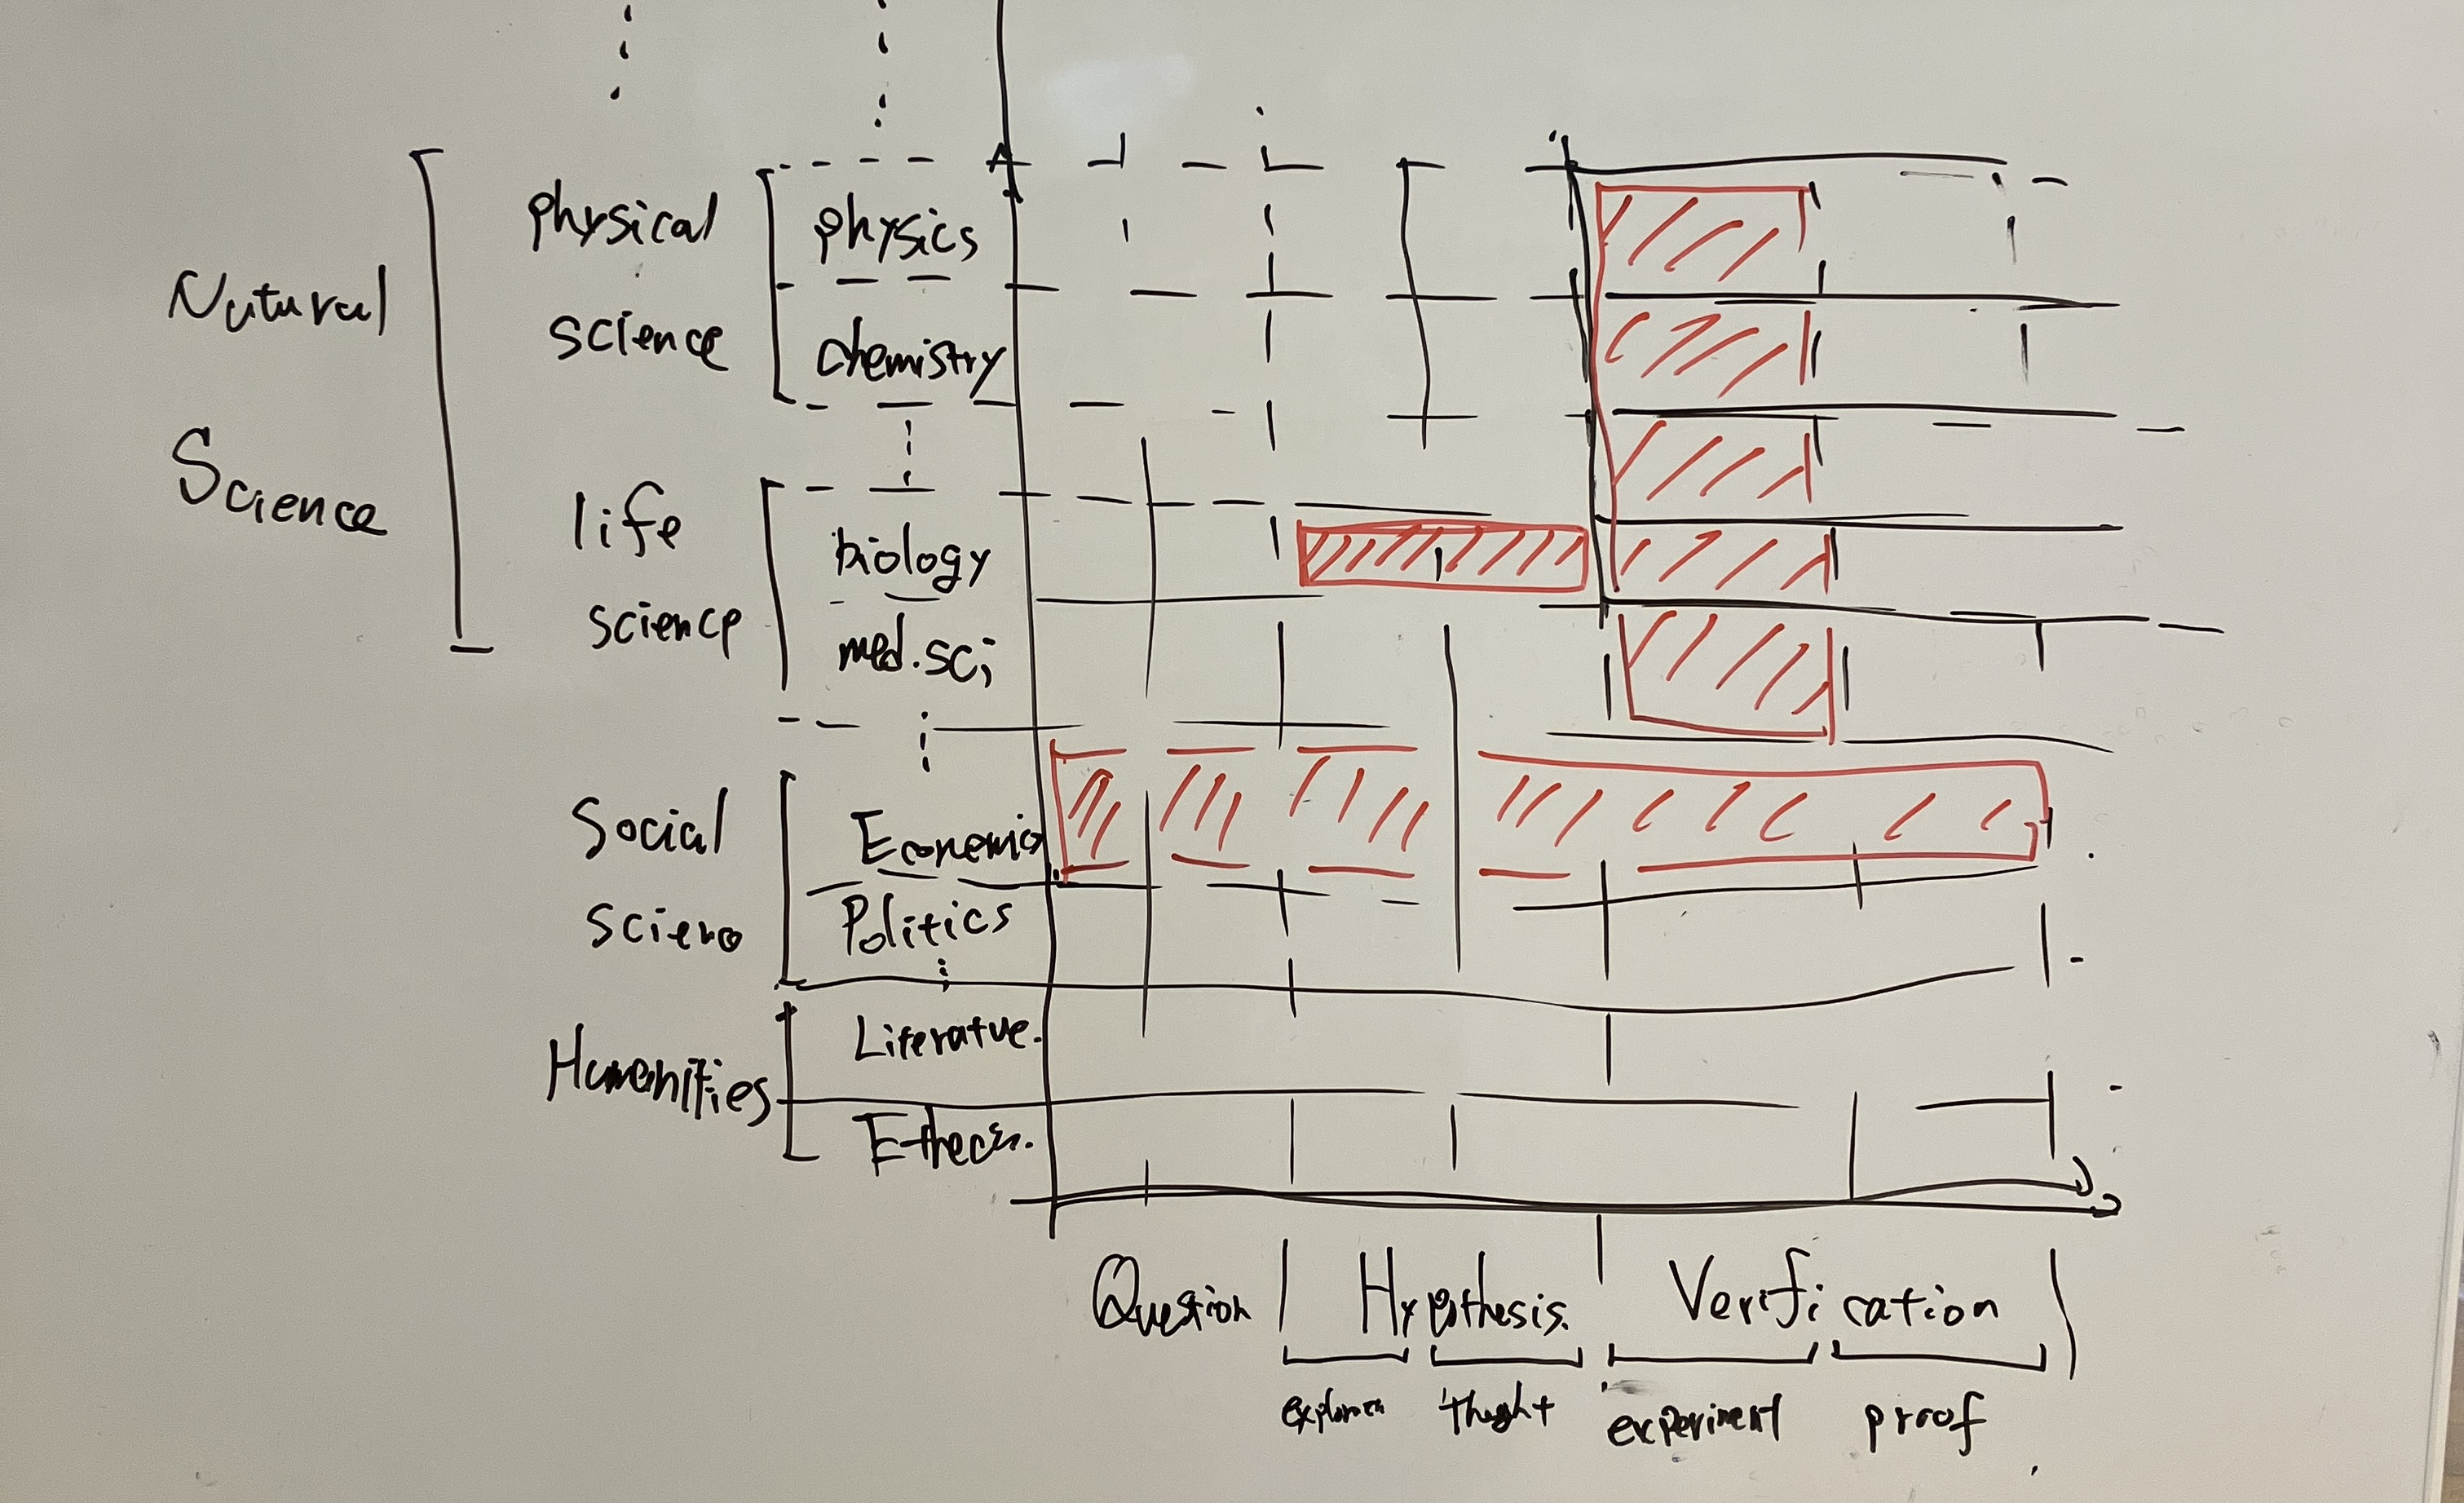
\includegraphics[width=\linewidth]{figs/generality_matrix.jpg}
    \caption{Caption}
    \label{fig:generality_matrix}
\end{figure}

Fig. \ref{fig:generality_matrix} conceptually illustrates the position of automation according to the axes of research field and research process. The vertical axis is the research field axis and the horizontal axis is the research process axis. Closer to the vertical axis corresponds to more specific research areas, and farther away from the vertical axis corresponds to a broader range of research areas. The horizontal axis corresponds to question construction, hypothesis generation, and hypothesis testing, from left to right, and is further divided within each category into more detailed e.g. empirical and non-empirical methods. Note that this is only a conceptual diagram and not an exact classification.

As a example, the automation of protein structure prediction \cite{jumper2021highly} can be seen as the automation of a certain hypothesis generation task in a certain molecular biology study. The work of robot scientist \cite{king2004functional} can also be understood as an attempt to automate many of the steps in the study of identifying the function of genes in genetics, from hypothesis generation, to testing, to generating new hypotheses. (Explanation of the figure).

Our goal of creating a versatile and autonomous artificial researcher is to automate everything on this two-dimensional surface. The area circled by the blue qualification in this figure corresponds to that. In other words, our goal is to realize an artificial intelligence that can autonomously execute any research or any process of research.

\section{Reviews and Perspectives}
So far, we have introduced each of the areas related to research automation. In this section, we will introduce review papers and perspective papers on research related to research automation. Note that the number of review papers on automation in individual research fields is too large to cover them all, so we have only selected review papers that are more comprehensive or abstract.

\subsubsection{Scientific Workflow}
Gill presents an extremely exciting idea of conducting automated research by turning the entire scientific process into compositional and modular software with the literature review of her and her colleagues' work. \cite{gil2022will}. For example, Gill et al. have created a software of the semantic workflow of scientific data analysis and computation process  \cite{gil2011semantic}. 
Each step of this workflow modularizes the procedures in research. Not only can these make analysis more efficient, but they also allow for the analysis of the research process itself. Furthermore, common workflows can be identified from multiple workflows, enabling abstraction of cross-domain knowledge about research process. Additionally, Gill and her team have proposed DISK, a systematic framework for hypothesis testing and data analysis. DISK can automatically cycle through a series of processes, including the generation of hypotheses, the determination of data and methods to test them, the acquisition of data from shared repositories, the analysis of that data, and the modification of hypotheses. Furthermore, each hypothesis is associated with information on confidence level and analysis details, which significantly indicates the plausibility of the hypothesis. Additionally, as the hypothesis and its confidence level and analysis are continuously updated and the revision history is retained, it enables the continuous maintenance and update of scientific findings.

\subsubsection{Nobel Turing Challenge}
Kitano also harbors an ambition to automate the entirety of the research process \cite{kitano2021nobel}. This is a thought-provoking paper that is meticulously contemplated. Kitano underscores the ability of AI in automating science to execute exhaustive and thorough exploration as a significant strength. We, as humans, aim to generate hypotheses that yield impactful results (Kitano refers to this as a value-driven approach). However, the importance of research findings is context-dependent, and research that we humans deemed unimportant may become crucial if the presuppositions or the context alter. Kitano proposes to eschew this value-driven approach and implement an alternative, exploration-driven methodology to science, aiming for novel scientific discoveries that were unattainable by human capabilities. Besides, Kitano with many examples and detailed consideration, presents a plethora of stimulating ideas, such as the continuous hypothesis network update, a roadmap to achieve autonomous artificial scientists, and proposition of the Nobel Turing Challenge as a Grand Challenge to substantially advance these endeavors. We highly encourage those interested to delve into this fascinating read.

\subsubsection{Task-guided Scientific Knowledge Retrieval}
Hope et al. have written a captivating perspective paper on the automation of research, presenting a fresh and exciting viewpoint \cite{hope2022computational}. They introduce a human-centric idea aimed at efficiently extracting relevant information from the ever-expanding body of research data, tailored specifically to the tasks researchers are engaged in - a framework they term \textit{task-guided scientific knowledge retrieval}. They start by conceptualizing the act of research as an interaction between a researcher's \textit{inner cognitive world} and the \textit{outer world}, or \textit{scientific ecosystem}. Building on this, they underscore the vital role of representing and retrieving information that aligns with the inner cognitive world of researchers, deftly transforming the cognitive functions used in human research into algorithmic processes.

Extensive discourse transpires concerning scientific discoveries. Yet, discussions pertaining to scientific comprehension remain relatively unexplored. Hope et al. delve into the conundrum of what it entails for a machine learning agent to not only unearth scientific knowledge but also to comprehend it \cite{krenn2022scientific}. They adopt a human-centric stance, positing that an agent's ability to offer explanations comprehensible to human scientists signifies the existence of its scientific understanding.

\section{Others}

Upon the completion of a study, the drafting of a manuscript, and its successful navigation of the peer-review process, the resulting findings are deemed to possess a degree of credibility as knowledge. Naturally, it would be hasty to assert that this alone births ``correct'' knowledge, as research demands iterative verification to confirm its validity. We convey such knowledge to others through various means, one of which is the presentation of research findings. To effectively communicate these outcomes, we create slides that elucidate our work. Studies also exist that strive to automate this aspect of the dissemination process \cite{sefid2019automatic}.

\section{Conclusion}